\documentclass[a4paper,12pt,line]{article}
% importing all the necessary packages before getting begin the document
\usepackage{color}
\usepackage{graphicx}
\usepackage[top=0in, bottom=0in, left=0.35in, right=0.85in]{geometry}
\usepackage{tikz}
\usepackage{tabularx}
\usepackage{hyperref}
\usepackage{colortbl}
\pagecolor{yellow!0}
\color{black}
\definecolor{rd}{RGB}{255,127,37}%manually defining a colour by giving RGB values
\pagestyle{empty}
\setlength{\parindent}{10ex}
\renewcommand{\baselinestretch}{1.5}


%initialising a document
\begin{document}
	
	%---------------------------- #1 ---------------------%
	%initialising space for creation of Top Red colour border>This is the theme of the Resume
	%-----------by drawing a rectangle filled with predefined color
	%using hspace to make the rectange to fit perfectly at the head of document
	\hspace*{-19mm}
	
\begin{tikzpicture}
		\draw [fill=rd,rd] (0,0) rectangle (19.4,0.5);
	\end{tikzpicture}
	\vspace*{3pt}
	
	
	%---------------------------- #2 ---------------------%
	%Name -- using color and Huge,LARGE size fonts and Bolded type of text
	%First name with full darkness in colour and Sur name at level 60 darkness
	%This is to differentiate The First name and Last name
	\begin{center}
		{\color{magenta}\Huge{\textbf{N}}\LARGE\textbf{\textrm{ISHANTH}}}\\
		\vspace{13pt}	
		{\color{magenta!60}\hspace{.8cm}\Huge{S}\LARGE\textsc{HANMUGAM}}\\
	\end{center}
	\vspace*{13pt}
	
	%---------------------------- #3 ---------------------%
	% Permanant address and contact information
	%Using flush left to allign the address to the left margin of the page
	%
	%-----Inserting profile pic at the declared location ,say (put(420,230))
	%and adjusting the width of the pic
	%
	%The pic should be stored in the location of this Program
	\begin{flushleft}
		5/309,	
		Rajiv gandhi nagar,\\
		Salem Road,\\
		Namakkal,\hspace{9.6cm}Mobile : +91-7200331572\\
		Tamilnadu.\hspace{9.5cm}E-mail : nishanthsnh@gmail.com\\
		
		\begin{picture}(0,0)
		\put(420,120){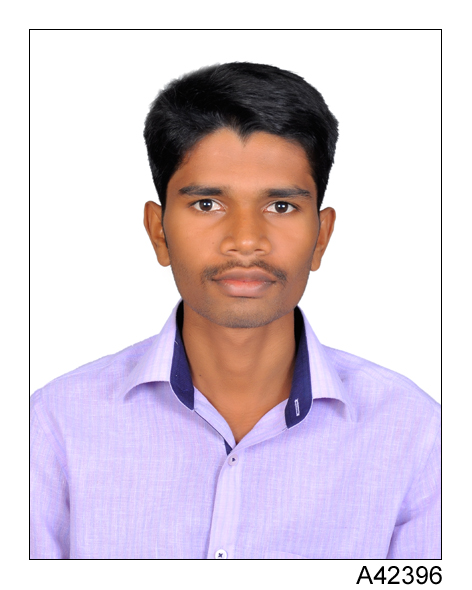
\includegraphics[width=30mm]{my.jpg}}
		\end{picture}
		
	\end{flushleft}
	\vspace{-15mm}

	%---------------------------- #4 ---------------------%
	%First section named as Objective with Magenta color
	\section*{\color{magenta}Objective}
	
		\hspace{10mm}To get and share my knowledge to the platform where I work, and to innovate an useful, service based idea for the growth of my Nation as well as my workplace
		
		
	%---------------------------- #5 ---------------------%
	
	%Initiation of table of 5 columns centered text with out vertical line
	%Colouring the row for highliting using colortbl package
	\section*{\color{magenta}Education}
	\begin{tabular}{ccccc}
		%\hline
		\rowcolor{yellow!20}
		\color{blue}\textsc{Degree}&\color{blue}\textsc{College/School}&\color{blue}\textsc{Board}&\color{blue}\textsc{Passing Year} &\color{blue}\textsc{Percentage}\\%\hline
		\rowcolor{orange!30}
		B.E(EIE)&M.Kumarasamy College of Engineering&Anna University&2017&8.1\textsuperscript{*}\\\rowcolor{orange!30}
		HSC&Bharathi higher secondary school&StateBoard&2013&86\\\rowcolor{orange!30}
		SSLC&Bharathi higher secondary school&StateBoard&2011&94\\
		
	\end{tabular}
	\begin{flushright}
		*upto 7th semester
	\end{flushright}

	%---------------------------- #6 ---------------------%
	%Third Section for Project details
	%--------------- Enumerated List #1 ------------------%
	\section*{{\color{magenta}Project}}
	\begin{enumerate}
		\item LASER SECURITY SYSTEM
		\item SECURITY SYSTEM USING GATES
		\item MULTIPLE SECURITY SYSTEM FOR APPLIANCES
		\item FACE RECOGNITION AND ATTENDANCE SYSTEM
		\item AUTONOMOUS CONTROL OF VEHICLE USING SPEED LIMIT SIGNS\\BASED ON IMAGE PROCESSING
	\end{enumerate}
	\vspace*{3.2cm}
	
	%---------------------------- #7 ---------------------%
	%Theme Completion of first page and creating new page
	\hspace{-1.9cm}
	
\begin{tikzpicture}
	\draw [fill=rd,rd] (0,0) rectangle (19.4,0.5);
	\end{tikzpicture}
	\newpage%creating page 2
	\hspace*{-19mm}
	
\begin{tikzpicture}
	\draw [fill=rd,rd] (0,0) rectangle (19.4,0.5);
	\end{tikzpicture}
		
		
	%---------------------------- #8 ---------------------%
	%Fourth section
	%Itemized list #1 for entering the Training and Internship
	
	\section*{{\color{magenta}Training and Internship}}
	\begin{itemize}
		\item PCB design training over a period of 5 days
		\item In plant training in EID PARRY SUGAR for a period of 5 days
		\item Basics of Distributed Control System of Yokagawa Systems for a period of 5 days
		
	\end{itemize}
		
	%---------------------------- #9 ---------------------%
	%Fifth section
	%Enumerated list #2 for entering Researh Publications details
	
	\section*{{\color{magenta}Research Publication}}
	
	\begin{enumerate}
		\item Published a paper on "GESTURE CONTROLLED HOME AUTOMATION USING IMAGE PROCESSING IN PYTHON" in final year of my course.
	\end{enumerate}
	
	%---------------------------- #10 --------------------%
	%Sixth Section
	%Itemized list #2 for entering Technical skill details
	
	\section*{{\color{magenta}Technical Skills}}
	\begin{itemize}
		\item Basic Circuit Designing
		\item Basics of C and Python programming languages
		\item Arduino Microcontroller programming
		\item Basics of Android app development in MIT app inventor
		\item Work with Proteus software for circuit design and simulation
	\end{itemize}
	
	%---------------------------- #11 --------------------%
	%Seventh Section
	%Enumerated list #3 for entering Soft skill details
	
	\section*{{\color{magenta}Soft Skills}}
	\begin{enumerate}
		\item Good Communication skill
		\item Adapdable to different environment
		\item Logic creation for problem solving
		\item Team worker with good managing skill
		\item Good learner
		\item Hard worker if involved in a work
	\end{enumerate}
	\vspace*{4.2cm}
	
\begin{tikzpicture}
	\draw [fill=rd,rd] (0,0) rectangle (19.4,0.5);
	\end{tikzpicture}
	%Page ends here also completion of theme for this page is done
	\newpage
	
	
	%---------------------------- #12 --------------------%
	%Eigth Section
	%Itemized list #3 for entering Extra Curricular Activities details
	%setting the same theme for this page
	\hspace*{-19mm}
	
\begin{tikzpicture}
	\draw [fill=rd,rd] (0,0) rectangle (19.4,0.5);
	\end{tikzpicture}
	\section*{{\color{magenta}Extra Curricular Activities}}
	\begin{itemize}
		\item Vice President of a NGO ‘THOLKODUPPOM’
		\item Active member in National Service Scheme
		\item Actively Participated in College March Past Troop
		\item Tamil poem writing
	\end{itemize}


	%---------------------------- #13 --------------------%
	%Ninth Section
	%Enumerated list #4 for entering Co-Curricular Activities details
	\section*{{\color{magenta}Co-Curricular Activities}}
	\begin{enumerate}
		\item Finished IWCF Level 1 Program,an online course which is meant for oil well safety
		\item Project Lead in 'TechExpo' an intra college Project display contest over Second,Third and final year
		\item Done Paper Presentations periodically
	\end{enumerate}


	%---------------------------- #14 --------------------%
	%Tenth Section
	%Itemized list #4 for entering Achievements details
	\section*{{\color{magenta}Achievements}}
	\begin{itemize}
		\item 1\textsuperscript{st} Prize in Project display held in Knowledge Institute of Technology,Salem,Tamilnadu.
		\item 1\textsuperscript{st} Prize in Circuit Debugging, held in Bannari Amman Institute of Technology,\\Sathyamanglam,Tamilnadu.
		\item 1\textsuperscript{st} Prize in Short film Contest in ORLIA’16,College Cultural meet 2016.
		\item 1\textsuperscript{st} in Tamil Poem writing in ORLIA'17,College cultural meet 2017.
		\item 2\textsuperscript{nd} Prize in Best Manager in ORLIA’15,College Cultural meet 2015.
		\item 3\textsuperscript{rd} Prize in Department level Project presentation at TECH EXPO’14.
	\end{itemize}


	%---------------------------- #14 --------------------%
	%Tenth Section
	%Itemized list #4 for entering Achievements details
	\section*{{\color{magenta}Languages Known}}
	\centering
	%\begin{tabular}{cc}
	\vspace{1pt}
	\color{blue}\textsc{Language} \hspace*{2cm}\color{blue}\textsc{Skill Level}\\
	\hspace*{0.7cm}\color{black}Tamil\hspace*{2.7cm}Read,Write,Speak\\
	\hspace*{0.7cm}English\hspace*{2.3cm}Read,Write,Speak\\
	\hspace*{-0.5cm}Hindi\hspace*{2.6cm}Read,Write\\
	%\end{tabular}
	
	\vspace*{1.5cm}
	
\begin{tikzpicture}
	\draw [fill=rd,rd] (0,0) rectangle (19.4,0.5);
	\end{tikzpicture}
	
	\newpage
	
\begin{tikzpicture}
	\draw [fill=rd,rd] (0,0) rectangle (19.4,0.5);
	\end{tikzpicture}
	
	%---------------------------- #15 --------------------%
	%Eleventh Section
	%Field to enter Personal Information
	%Uses a tabular method for creation
	\begin{flushleft}
		\section*{{\color{magenta}Personal Information}}
		%\hspace{1cm}
		\begin{tabular}{lcl}
			Father's Name&:&Shanmugam M\\
			Mother's Name&:&Shanmugavalli S\\
			Age&:&21\\
			Date of Birth&:&29.06.1996\\
			Gender&:&Male\\
			Nationality&:&Indian\\
		\end{tabular}
	
	
	%---------------------------- #16 --------------------%
	%Twelvth Section
	%Field to enter Reference
	%Uses a bolded font style
	\section*{{\color{magenta}Reference}}
	\textbf{
		Dr.J.UMA\\
		Head - Department of Electronics \& Instrumentation Engineering\\
		M.Kumarasamy College of Engineering\\
		Karur,Tamilnadu\\
		Ph:04324 - 270755 / 272155\\
		Email : hodeie@mkce.ac.in\\}
	
	%---------------------------- #17 --------------------%
	%Thirteenth Section
	%Field to enter Declaration
	{\color{yellow} \rule{\linewidth}{0.8mm} }%drawing a line of defined thickness
	\vspace{-1.5cm}
	\section*{{\color{magenta}Declaration}}
	
	\hspace{1cm}I hereby declare that the details furnished above are true and correct to the best of my knowledge
	and belief and I undertake to inform you of any changes therein, immediately.
	for it. 
	\vspace{5mm}
	{\color{yellow} \rule{\linewidth}{0.8mm} }
	\end{flushleft}


	%---------------------------- #18 --------------------%
	%Fourteenth Section
	%Finishing off the document by entering Date and Signature Space
	%Theme gets completed
	\vspace*{7.5cm}
	\textbf{Date: \hspace*{12cm}Signature}\\
	\vspace*{10mm}
	
\begin{tikzpicture}
	\draw [fill=rd,rd] (0,0) rectangle (19.4,0.5);
\end{tikzpicture}
\end{document}